
% You may delete everything from \appendix up to \end{document} if you don't need it.
\appendix

\chapter{Appendix}

\section{Histogram over Incorrect Region Lengths}\label{app:histogram_over_region_lengths}

\begin{figure}[h]
    \centering
    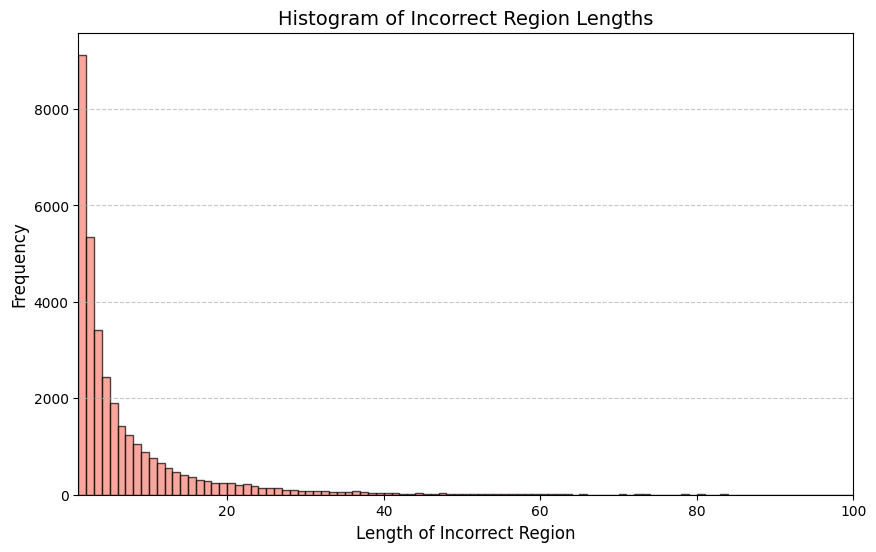
\includegraphics[width=0.6\textwidth]{figures/incorrect_region_histogram.png}
    \caption{Histogram over incorrect region lengths. The incorrect region distribution has a long-tail, with $26.7\%$ regions being of length 1. This raises concerns over the smoothness of outputs and requires some form of post-processing explored in Section~\ref{sec:decoding}.}
    \label{fig:histogram_over_region_lengths}
\end{figure}

\newpage

\section{Accuracy vs Context Length of Evaluation}\label{app:accuracy_vs_context_length}

\begin{figure}[h]
    \centering
    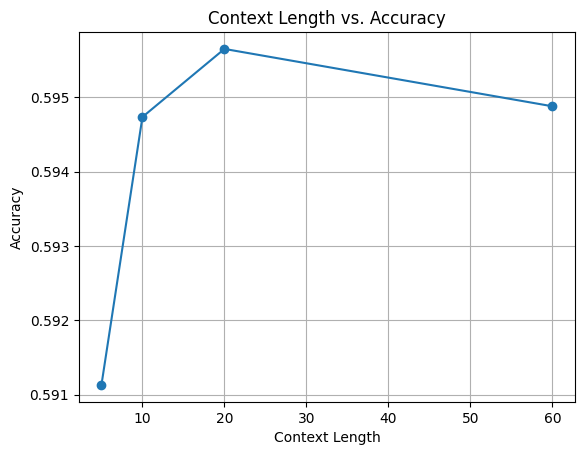
\includegraphics[width=0.5\textwidth]{figures/context_length_vs_accuracy.png}
    \caption{Accuracy vs context length of evaluation. The accuracy increases very slightly. The effect size is so small that we conclude it does not make a difference, and choose to evaluate over the entire song at once.}
    \label{fig:accuracy_vs_context_length}
\end{figure}

\section{Accuracy vs Hop Length}\label{app:accuracy_vs_hop_length}

\begin{figure}[h]
    \centering
    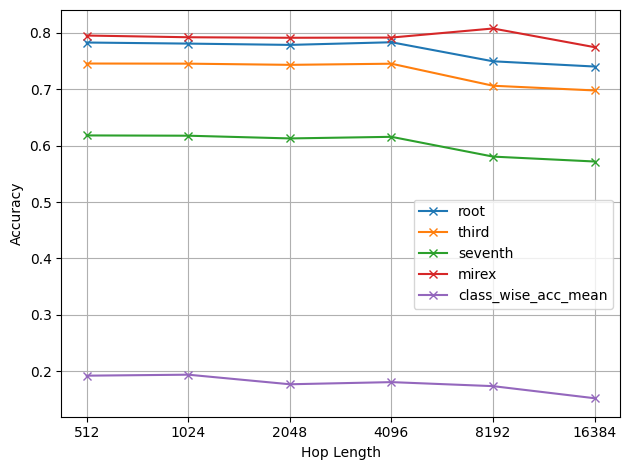
\includegraphics[width=0.5\textwidth]{figures/hop_length_vs_accuracy.png}
    \caption{Accuracy vs hop length. Metrics are not directly comparable over hop lengths due to different likelihoods. However, the metrics are fairly consistent over different hop lengths, certainly over the region explored by the literature $[512,2048,4096]$. Every hop length tested is short enough to be more granular than chords, but not so short that the computed CQT is too noisy. We continue with the default hop length of $4096$, to be consistent with some of the literature while keeping computational cost low.}
    \label{fig:accuracy_vs_hop_length}
\end{figure}